\documentclass{beamer}

\usepackage{ctex}
\usepackage{subfigure}
\usepackage{multicol}
\usepackage{bm}

\useinnertheme{rectangles}

\xdefinecolor{xjtured}{RGB}{200,22,30}
\xdefinecolor{xjturedbak}{RGB}{184,0,46}
\xdefinecolor{xjtublue}{RGB}{0,78,151}
\xdefinecolor{xjtubluebak}{RGB}{0,46,230}
\xdefinecolor{xjtugrey}{RGB}{220,220,221}
\xdefinecolor{xjtugreybak}{RGB}{92,54,9}

\setbeamercolor{structure}{bg=xjtublue}
\setbeamercolor{title}{fg=white}
\setbeamercolor{section in head/foot}{fg=white,bg=xjtublue}
\setbeamercolor{subsection in head/foot}{fg=white,bg=xjtubluebak}
\setbeamercolor{frametitle}{fg=xjtublue,bg=xjtugrey}
\setbeamercolor{author in head/foot}{fg=white,bg=xjtublue}
\setbeamercolor{title in head/foot}{fg=white,bg=xjtublue}
\setbeamercolor{block title}{fg=white,bg=xjtubluebak}
\setbeamercolor{block body}{bg=block title.bg!10!white}
\setbeamercolor{block title example}{fg=white,bg=green}
\setbeamercolor{block body example}{bg=block title example.bg!10!white}
\setbeamercolor{block title alerted}{fg=white,bg=red}
\setbeamercolor{block body alerted}{bg=block title alerted.bg!10!white}
\setbeamercolor{item projected}{bg=xjtublue}
\setbeamercolor{subitem projected}{bg=xjtublue}

\setbeamertemplate{footline} 
{%
  \begin{beamercolorbox}[ht=2.5ex,dp=1.125ex,%
    leftskip=.3cm,rightskip=.3cm]{title in head/foot}%
    {\insertshorttitle}%
    \hfill%
    {\insertframenumber / \inserttotalframenumber}
  \end{beamercolorbox}%
}

% \logo{
\includegraphics[height=10cm]{figures/a3_3jdxhgray.png}}

\begin{document}

\AtBeginSection[]
{
  \begin{frame}
    \tableofcontents[currentsection,hideallsubsections]
  \end{frame}
}
\AtBeginSubsection[]
{
  \begin{frame}
    \tableofcontents[currentsection,currentsubsection]
  \end{frame}
}

\title{Seminar One}
\author{DX}
\institute{XJTU}
\begin{frame}
  \titlepage
\end{frame}

\begin{frame}
  \frametitle{Outline}
  \tableofcontents %  [pausesections]
\end{frame}

\section{Topic One}
\subsection{Converter Valve}
\begin{frame}{Structure}
  \begin{figure}
    \subfigure[Real Image]{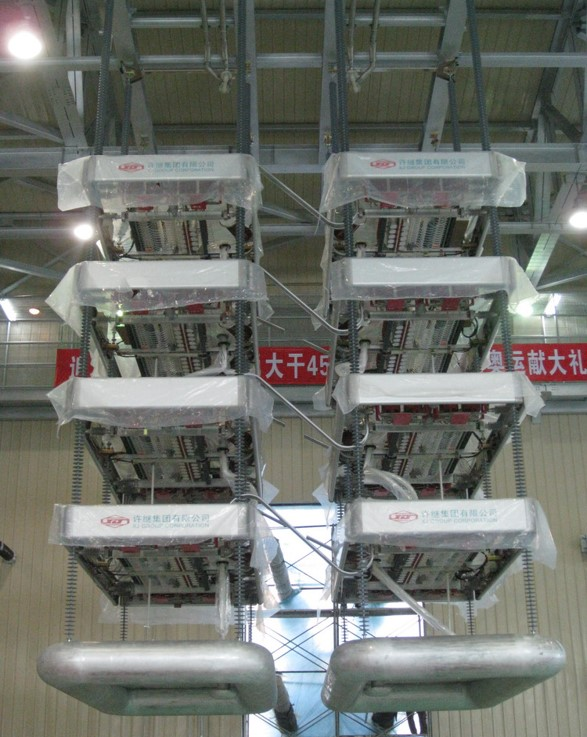
\includegraphics[clip=true,height=4.2cm]{figures/realimg}}\qquad
    \subfigure[Structure]{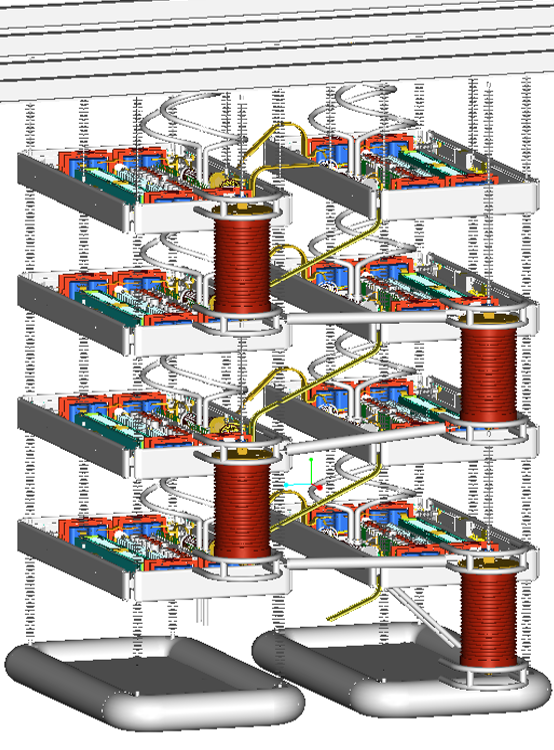
\includegraphics[clip=true,height=4.2cm]{figures/structure}}
    \caption{Converter Valve}
  \end{figure}
\end{frame}

\begin{frame}{Layer}
  \begin{figure}
    \centering
    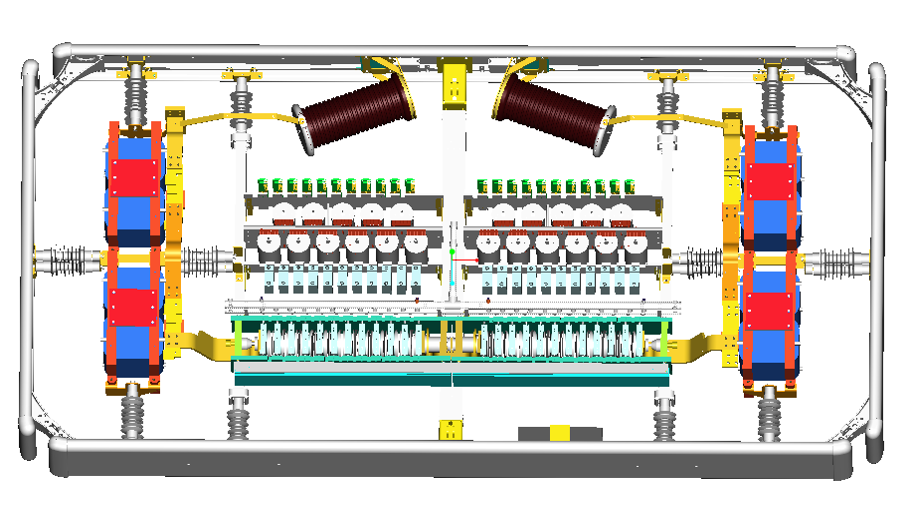
\includegraphics[width=0.8\textwidth]{figures/layer}
    \caption{Layer}
  \end{figure}
\end{frame}

\begin{frame}{Circuit}
  \begin{figure}
    \centering
    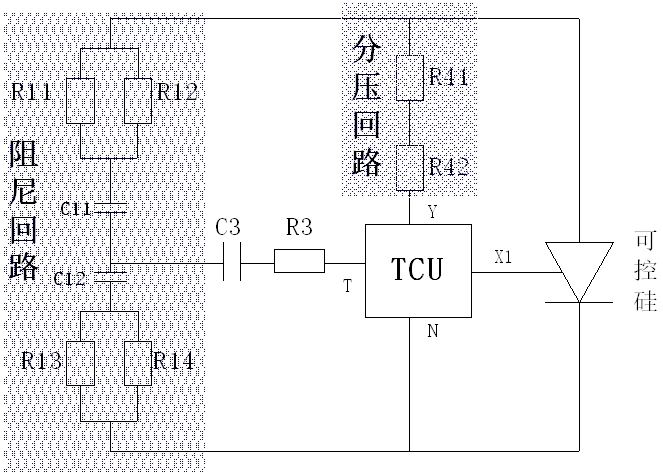
\includegraphics[width=0.6\textwidth]{figures/circuit}
    \caption{Basic Circuit}
  \end{figure}
\end{frame}

\section{Electromagnetic Field}
\subsection{Maxwell}
\begin{frame}{Maxwell Equation}
  \begin{columns}
    \begin{column}{0.55\textwidth}
      \begin{align*}
        &\oint_l\vec{H}\cdot\mathrm{d}l=\int_S\vec{J}\cdot\mathrm{d}S+\int_S \frac{\partial\vec{D}}{\partial t}\cdot\mathrm{d}S \\
        &\oint_l\vec{E}\cdot\mathrm{d}l=-\int_S\frac{\partial\vec{B}}{\partial t}\cdot\mathrm{d}S \\
        &\oint_S\vec{B}\cdot\mathrm{d}S=0 \\
        &\oint_S\vec{D}\cdot\mathrm{d}S=q \\
      \end{align*}
    \end{column}
    \begin{column}{0.45\textwidth}
      \begin{block}{关系}
        \begin{align*}
          &\vec{D}=\epsilon\vec{E} \Rightarrow \mbox{类似电容的关系} \\
          &\vec{B}=\mu\vec{H} \Rightarrow \mbox{类似电感的关系} \\
          &\vec{J}=\gamma\vec{E} \Rightarrow \mbox{类似电阻的关系} \\
        \end{align*}
      \end{block}
    \end{column}
  \end{columns}
\end{frame}

\subsection{Transmission Line}
\begin{frame}{Telegrapher's Equation}
  \begin{columns}
    \begin{column}{0.45\textwidth}
      \begin{figure}
        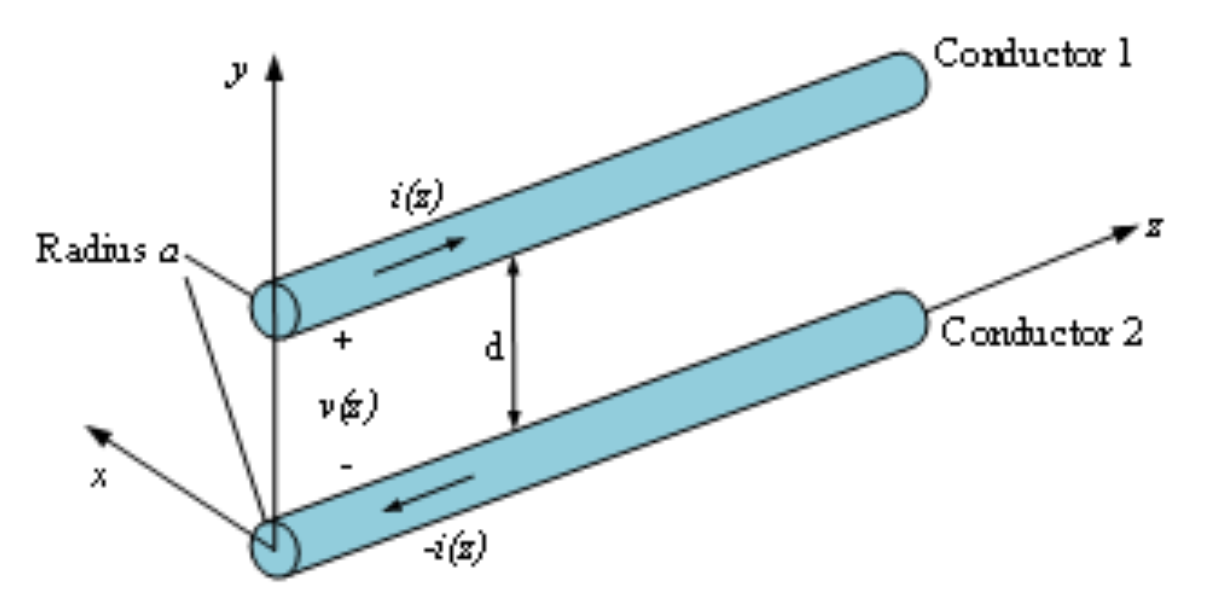
\includegraphics[width=\textwidth]{figures/transmission}
      \end{figure}
    \end{column}
    \begin{column}{0.55\textwidth}
      \begin{align*}
        &-\frac{\partial v(z,t)}{\partial z}=\mathop{R'}i(z,t)+\mathop{L'}\frac{\partial i(z,t)}{\partial z} \\
        &-\frac{\partial i(z,t)}{\partial z}=\mathop{G'}v(z,t)+\mathop{C'}\frac{\partial v(z,t)}{\partial z} \\
      \end{align*}
    \end{column}
  \end{columns}
\end{frame}

\section{third section}
\begin{frame}
  \frametitle{3}
  test information
\end{frame}

\end{document} 